
%(BEGIN_QUESTION)
% Copyright 2013, Tony R. Kuphaldt, released under the Creative Commons Attribution License (v 1.0)
% This means you may do almost anything with this work of mine, so long as you give me proper credit

Suppose we have a Siemens S7-200 PLC connected to a pair of momentary-contact pushbutton switches and a light bulb as shown in this illustration:

$$\includegraphics[width=15.5cm]{i03360x01.eps}$$

Examine the following relay ladder logic (RLL) program for this Siemens PLC, determining the statuses of the two lamps provided both switches are simultaneously pressed by a human operator:

$$\includegraphics[width=15.5cm]{i03360x02.eps}$$

Complete the following ``truth table'' showing the status of the light bulb given all possible switch status combinations:

% No blank lines allowed between lines of an \halign structure!
% I use comments (%) instead, so that TeX doesn't choke.

$$\vbox{\offinterlineskip
\halign{\strut
\vrule \quad\hfil # \ \hfil & 
\vrule \quad\hfil # \ \hfil & 
\vrule \quad\hfil # \ \hfil \vrule \cr
\noalign{\hrule}
%
% First row
Switch A & Switch B & Light Bulb \cr
%
\noalign{\hrule}
%
% Another row
Unpressed & Unpressed & \cr
%
\noalign{\hrule}
%
% Another row
Unpressed & Pressed & \cr
%
\noalign{\hrule}
%
% Another row
Pressed & Unpressed & \cr
%
\noalign{\hrule}
%
% Another row
Pressed & Pressed & \cr
%
\noalign{\hrule}
} % End of \halign 
}$$ % End of \vbox

\underbar{file i03360}
%(END_QUESTION)





%(BEGIN_ANSWER)

% No blank lines allowed between lines of an \halign structure!
% I use comments (%) instead, so that TeX doesn't choke.

$$\vbox{\offinterlineskip
\halign{\strut
\vrule \quad\hfil # \ \hfil & 
\vrule \quad\hfil # \ \hfil & 
\vrule \quad\hfil # \ \hfil \vrule \cr
\noalign{\hrule}
%
% First row
Switch A & Switch B & Light Bulb \cr
%
\noalign{\hrule}
%
% Another row
Unpressed & Unpressed & Off \cr
%
\noalign{\hrule}
%
% Another row
Unpressed & Pressed & Off \cr
%
\noalign{\hrule}
%
% Another row
Pressed & Unpressed & On \cr
%
\noalign{\hrule}
%
% Another row
Pressed & Pressed & On \cr
%
\noalign{\hrule}
} % End of \halign 
}$$ % End of \vbox

\vskip 10pt

Note how Switch B has no effect on the PLC's output status!  The reason for this is the placement of the two identically-addresses coils in the PLC program: each rung writes either a 0 or a 1 to the same output bit {\tt Q0.1}, but only the {\it last} rung's state is in effect when the PLC finishes its scan of the program and updates the output registers to actually turn its output channels on or off.

This is why it is a bad idea to assign the same address to multiple coils in a PLC program, the only exception to this rule being when the coils in question are retentive (i.e. ``Set'' and ``Reset'' or ``Latch'' and ``Unlatch'' coils) in which case complementary coil pairs bearing the same address is proper.  Regular, non-retentive coil instructions, however, will conflict with one another in a PLC program if they bear the same bit address.

%(END_ANSWER)





%(BEGIN_NOTES)


%INDEX% PLC, relating I/O status to virtual elements

%(END_NOTES)


